\hypertarget{experiments}{
}

In the experimental stage of this research, four experiments are performed on two different datasets to analyse the overall quality of the synthesized data. The experiments conducted by Targhi for diffuse material classes are replicated and extended with synthesis using other reflection models, and the same setup is used on a new selection of material classes from the {\it PhoTex} database. The new selection of material classes have more specular properties unlike the classes selected by Targhi, which should give a better indication for the quality of specularity simulated by Phong, Blinn-Phong and Cook-Torrance reflectance.

\section{Preprocessing}\label{sec:preprocessing}
The {\it PhoTex} database consists of images recorded under a fixed point of view with varying light-source directions registered for each image. All images have a fixed size of $512 \times 512$ pixels. For the experiments, two datasets are chosen: a dataset according to the selection made by Targhi and another dataset with shiny properties to extend the experiments for the specular reflection models.

After rendering new images for the materials and before extracting the features from the materials, the rendered images are set to zero-mean and unit-variance in order to make the features intensity-invariant.

\subsection{Diffuse material classes}
Since we are interested in reproducing some results from the experiments of Targhi, and measure performance of more complex reflection models with respect to the Lambertian reflection model he applied, we need to select the same material classes he used in his experiment. These material classes are shown in figure \ref{fig:PhoTexData}.

From each material class, 40 images with certain slant and tilt angles are selected. The selected slant angles are $\{30^0, 45^0,60^0,75^0\}$. The images under a slant of $30^0$ have four different tilts, $\{0^0, 90^0, 180^0, 270^0\}$. The images with slants $\{45^0,60^0,75^0\}$ have tilts of $\{0^0,30^0,60^0,..., 300^0,330^0\}$. 

\subsection{Shiny material classes}
Because three out of five reflection models simulate specularity only, the previous dataset might not be good enough to measure improvements made by these reflection models. For this reason, a new dataset is selected from the {\it PhoTex} database with more specular properties. 

The material classes selected are shown in figure X. This dataset consists of 10 material classes, recorded under a slant of $75^0$ and tilts of $0^0$ to $350^0$ in increments of $10^0$, giving a total of 36 images for each material class.


\section{Reflection model parameters}\label{sec:ParameterSetting}
The reflection models used in the process of synthesis need material dependent parameters to be set, such as the parameter for the specular lobe size or surface roughness. However, these parameters are not available for the materials in the database in case of the micro-facet models, and in case of the empirical models there are no known 'good' values for the parameters to be set. To set these values, the parameters are computed using a gradient descent procedure with a total sum of squares error estimation:

		\begin{eqnarray*}
			Err(A,A') = \sum_{i=1}^n (a_i - a_i')^2
		\end{eqnarray*}
 
Where $A$ is the original image from the {\it PhoTex} database, and $A'$ is the synthesized image. By calculating the squared error per-pixel from the original image and the synthesized image, and accumulate the error over all pixels, an estimation of the total error serves as an indicator for the gradient descend. Both images are preprocessed to have zero-mean and unit-variance before the error is calculated, since the features will be extracted from preprocessed images.

Because the number of materials and the number of parameters to be estimated for each reflection model turn out to be large in total, a simplified gradient descend is done. Each parameter is estimated using a defined range of possible values. For the microfacet models, the roughness of a material could be $m \in \{0.1, 0.3, 0.5, 0.7, 0.9\}$ and the Fresnel coefficient in $R_f \in \{0.01, 0.03, 0.05, 0.07, 0.09\}$. The shininess constant for Phong and Blinn-Phong reflection could be $\alpha \in \{0.01, 10.0, 50.0\}$, and the material . 

The albedo and surface normals needed for this procedure are derived for each material from images with light directions registered with a slant of $30^0$ and tilts of $\{0^0, 90^0, 180^0, 270^0\}$. The choice for this configuration of angles over the hemisphere is based on the quality of the recovered surface albedo and surface normals and the . Using many images for photometric stereo give rise to many outliers such as speculars in the albedo. With a uniform choice of angles over the hemisphere, these outliers have minimal influence.

%\begin{comment}
\begin{figure}[h]
	\begin{center}
		\subfigure[aaa]{
\epsfig{file=images/db/aaa.eps, width=0.15\linewidth}}
		\subfigure[aab]{
\epsfig{file=images/db/aab.eps, width=0.15\linewidth}}
		\subfigure[aaj]{
\epsfig{file=images/db/aaj.eps, width=0.15\linewidth}}
		\subfigure[aam]{
\epsfig{file=images/db/aam.eps, width=0.15\linewidth}}
		\subfigure[aan]{
\epsfig{file=images/db/aan.eps, width=0.15\linewidth}}

		\subfigure[aao]{
\epsfig{file=images/db/aao.eps, width=0.15\linewidth}}
		\subfigure[aar]{
\epsfig{file=images/db/aar.eps, width=0.15\linewidth}}
		\subfigure[aas]{
\epsfig{file=images/db/aas.eps, width=0.15\linewidth}}
		\subfigure[aba]{
\epsfig{file=images/db/aba.eps, width=0.15\linewidth}}
		\subfigure[abj]{
\epsfig{file=images/db/abj.eps, width=0.15\linewidth}}

		\subfigure[abk]{
\epsfig{file=images/db/abk.eps, width=0.15\linewidth}}
		\subfigure[acc]{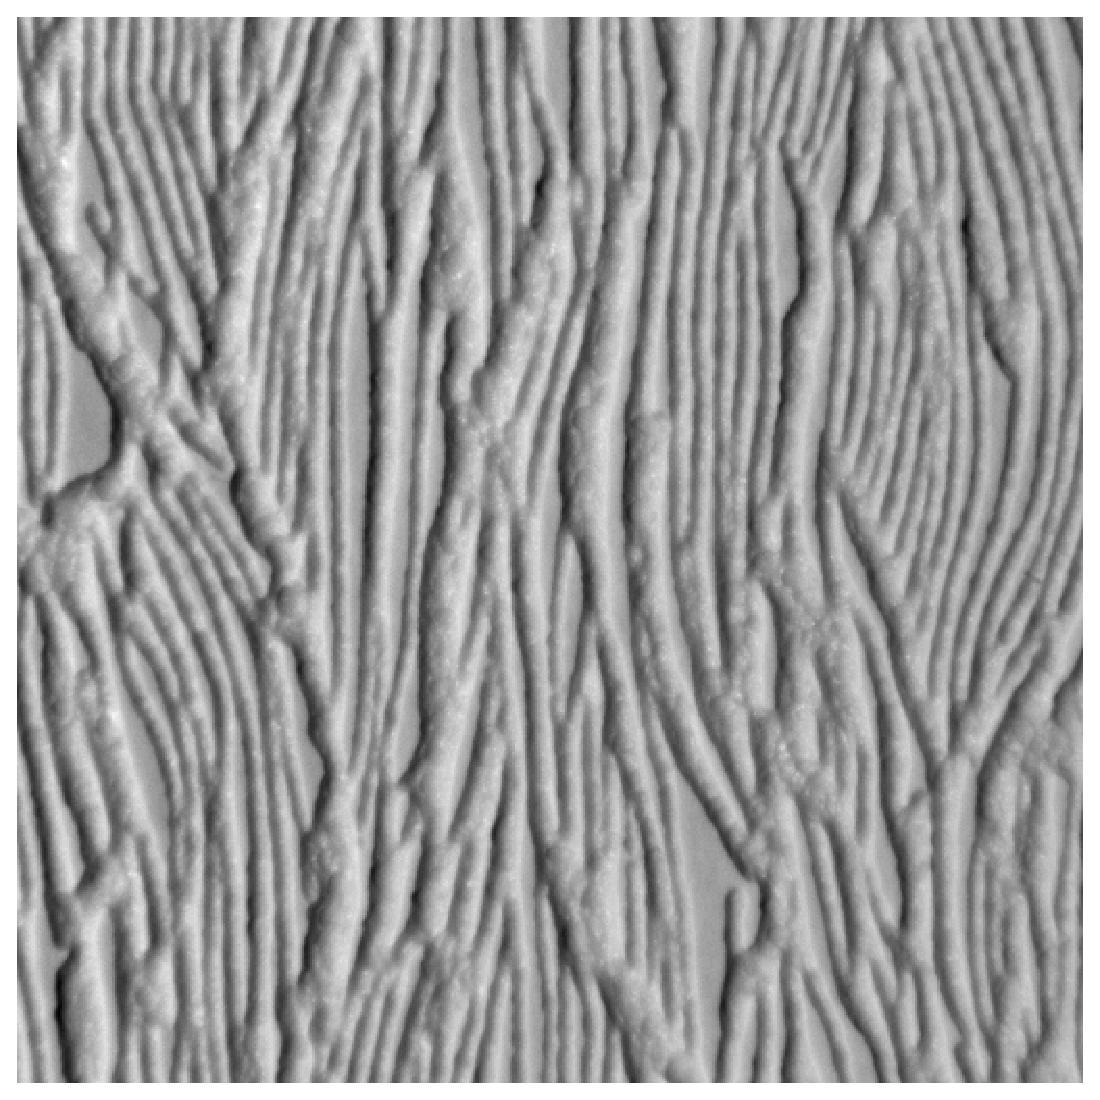
\epsfig{file=images/db/acc.eps, width=0.15\linewidth}}
		\subfigure[acd]{
\epsfig{file=images/db/acd.eps, width=0.15\linewidth}}
		\subfigure[ace]{
\epsfig{file=images/db/ace.eps, width=0.15\linewidth}}
		\subfigure[adb]{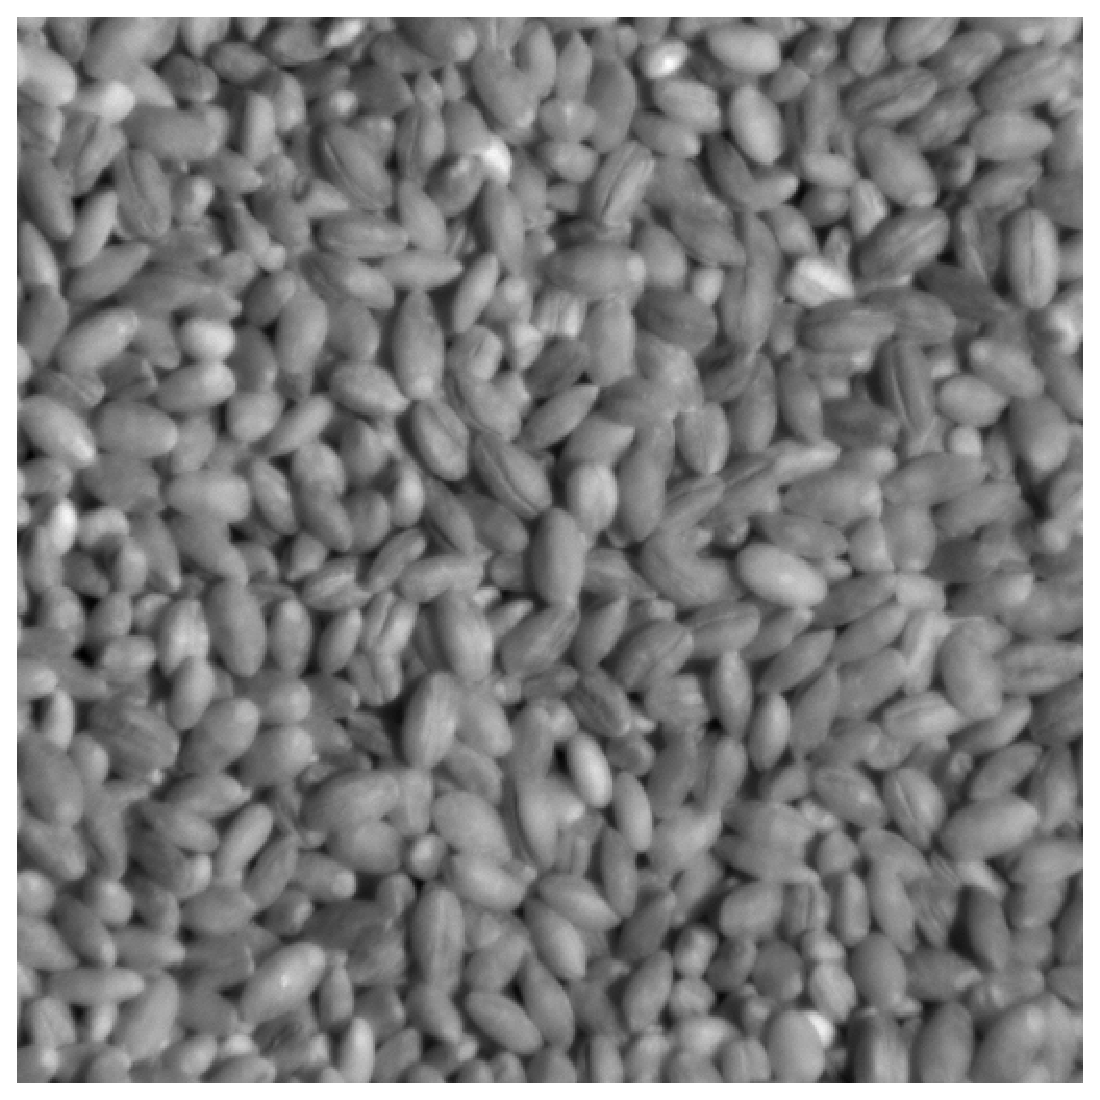
\epsfig{file=images/db/adb.eps, width=0.15\linewidth}}

		\subfigure[adc]{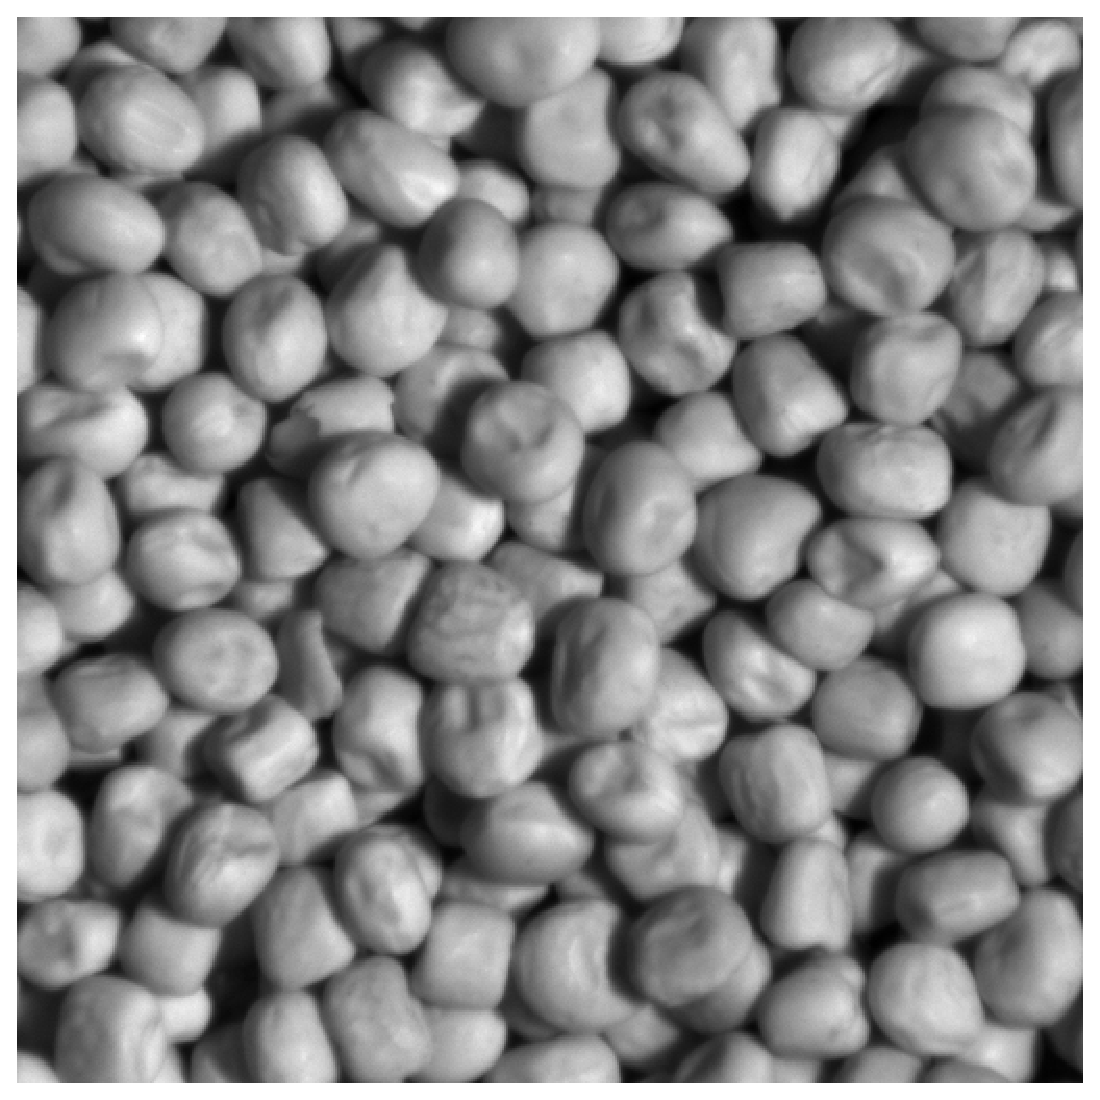
\epsfig{file=images/db/adc.eps, width=0.15\linewidth}}
		\subfigure[add]{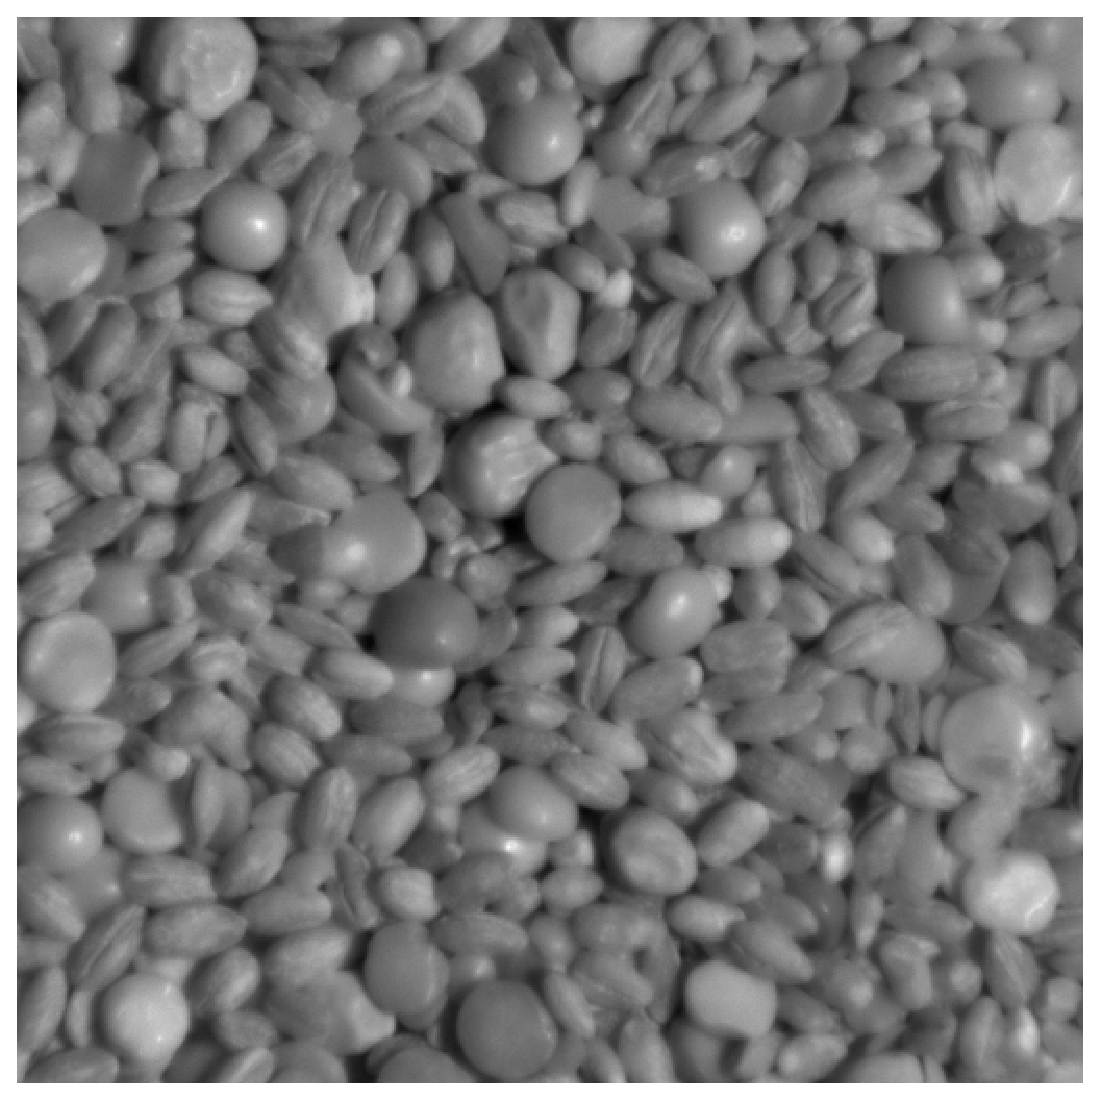
\epsfig{file=images/db/add.eps, width=0.15\linewidth}}
		\subfigure[ade]{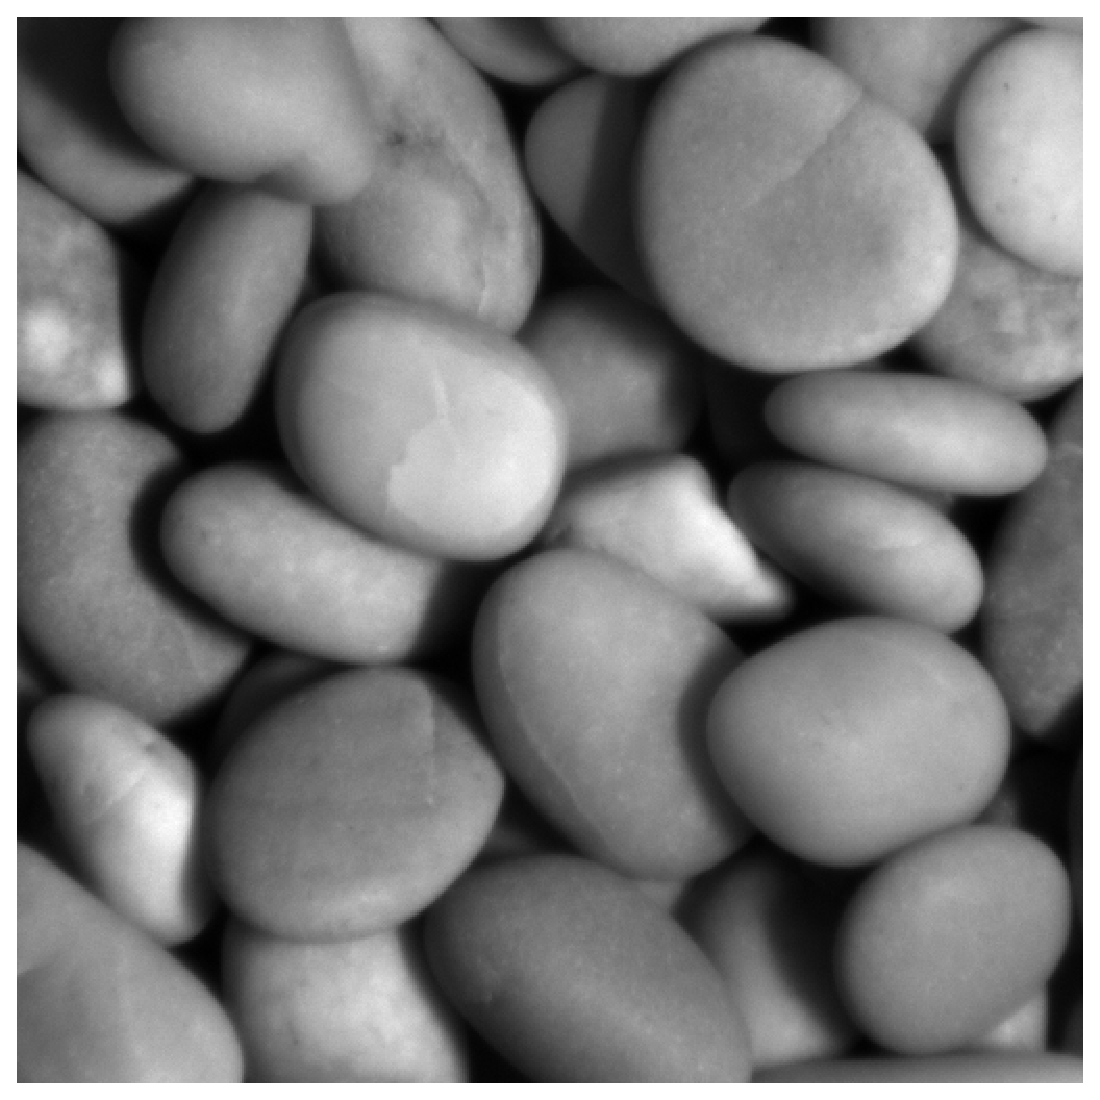
\epsfig{file=images/db/ade.eps, width=0.15\linewidth}}
		\subfigure[adg]{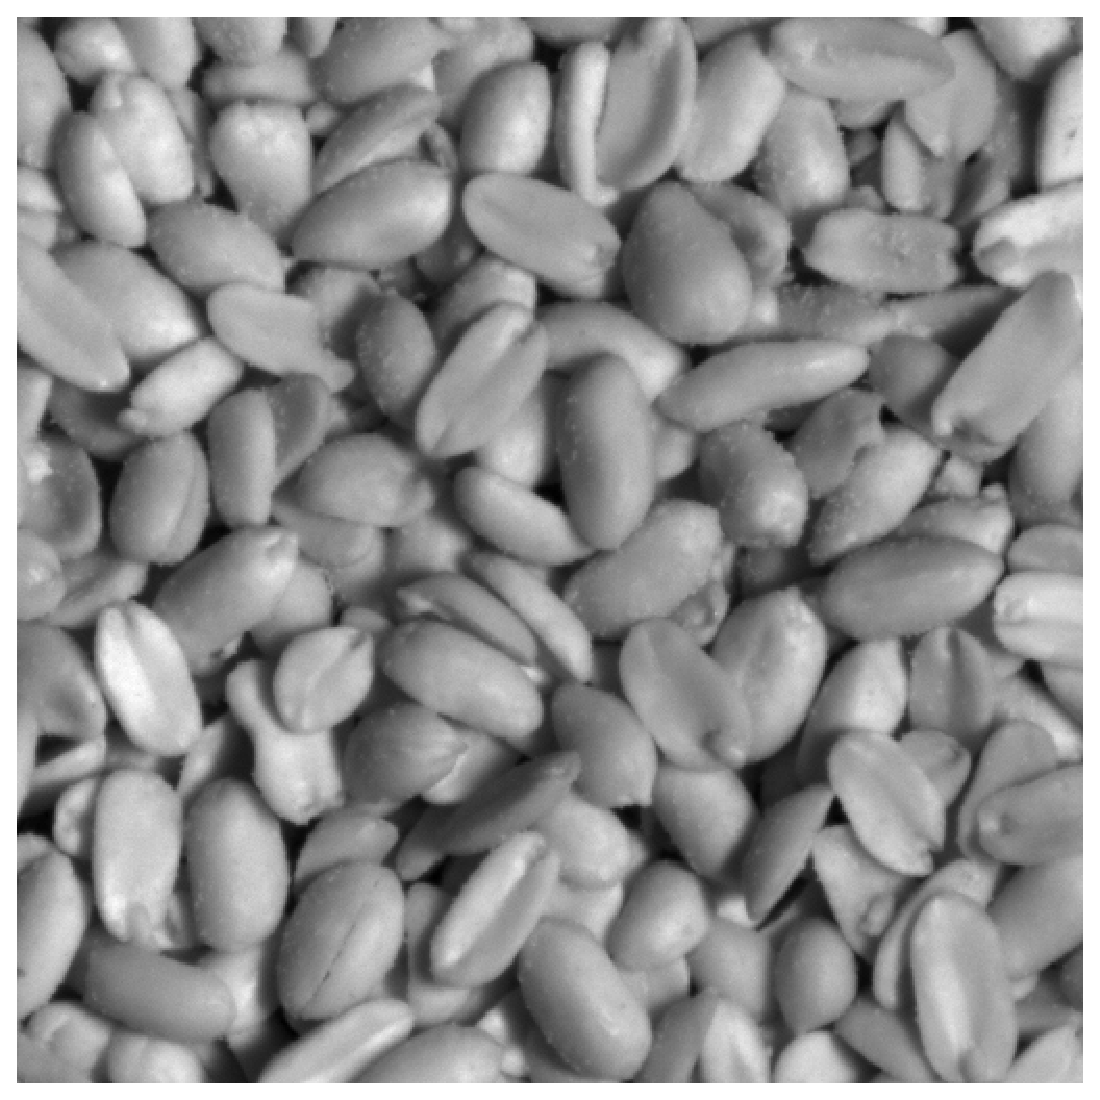
\epsfig{file=images/db/adg.eps, width=0.15\linewidth}}
		\subfigure[adh]{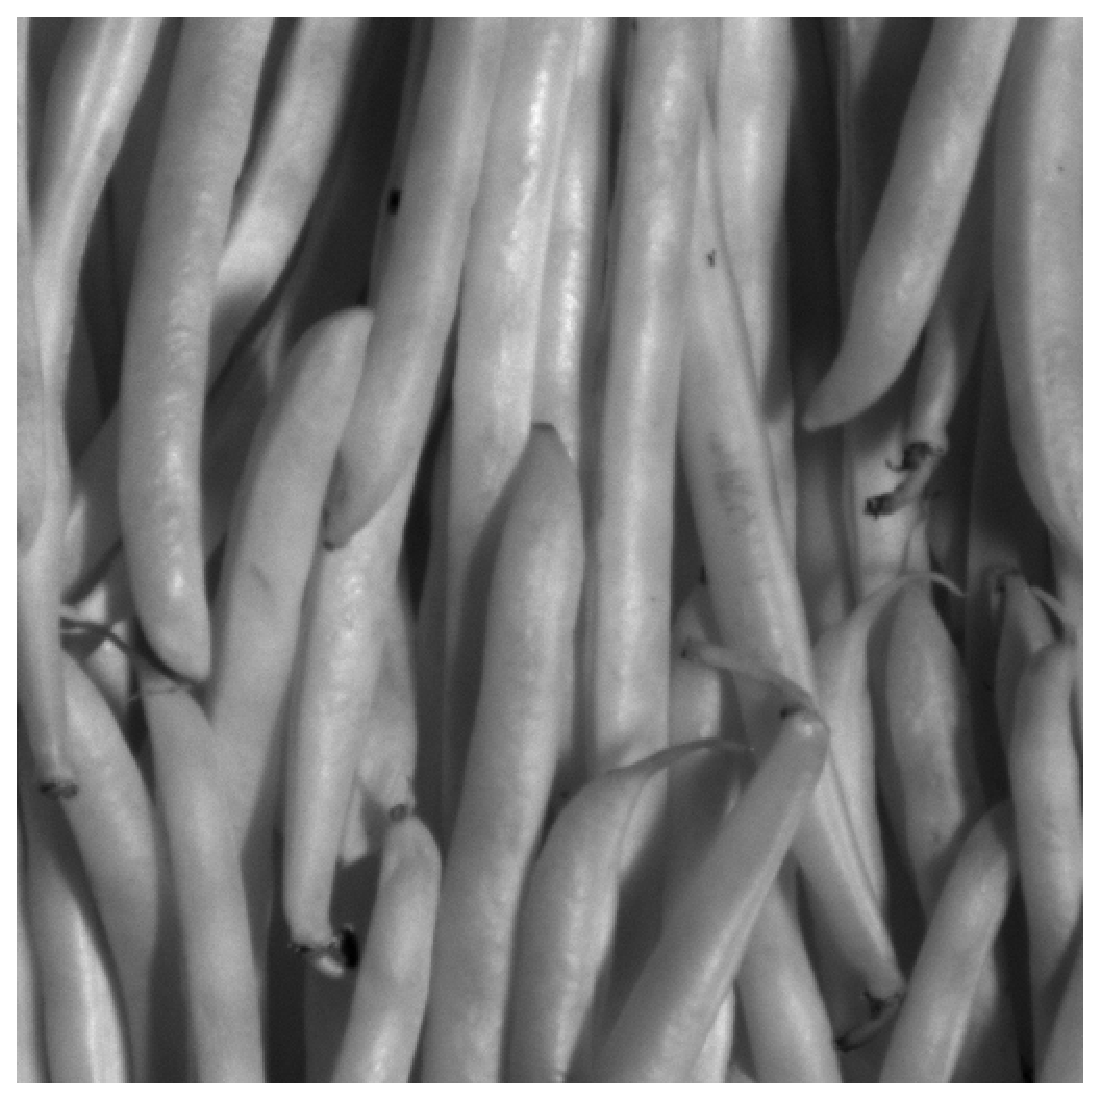
\epsfig{file=images/db/adh.eps, width=0.15\linewidth}}
	\end{center}
	\caption{{\it The material classes taken from the PhoTex database. The example images are registered under a slant of $30^0$ and a tilt of $0^0$.}}
	\label{fig:PhoTexData}
\end{figure}
%\end{comment}


\section{Experimental Setup}\label{sec:Experiments}
From the 40 images of each material class, 20 are selected for the training set, and the remaining are selected for the test set. Four different training sets are considered. These training sets are meant to be used for photometric stereo to compute the albedo and surface normals. Listed are the number of images used for this procedure for each class separately:

\begin{itemize}
	\item{\textit{T1} - the 20 images selected for training initially}
	\item{\textit{T2} - 10 randomly selected images from \textit{T1}}
	\item{\textit{T3} - 4 randomly selected images from \textit{T1}}
	\item{\textit{T4} - 3 randomly selected images from \textit{T1}. The minimum amount of images needed for photometric stereo.}
\end{itemize}

In Targhi's experiments, he devised different sets of generated data. The first set, $G1$, mimics the images used for photometric stereo. This means that for $T1$, the set $G1$ will consist of 20 images synthesized for each class, all with the light-directions equal to that of the registered directions of the images in $T1$. For $T2$, the set of $G1$ consists of 10 synthesized images for each class, and the same analogy applies for $T3$ and $T4$. This experiment is replicated and similar accuracies were measured.

The exact results from Targhi's experiment are hard to replicate since the quality of the synthesized image data depends strongly on the procedure of photometric stereo and its input. Since he uses a pseudo-random selection procedure to obtain the T1 set, where pseudo-random is defined as selecting slant and tilt angles to be uniform over the hemisphere, it is hard to obtain the same dataset. 

Pseudo-random in this research is defined as follows: for every slant, a number of tilts is available. There are three configurations of tilts possible such that the hemisphere is covered uniformly when using tilts in increments of $90^o$. To select the 20 images for each class, 5 slants are chosen randomly, and for each slant, a configuration of 4 tilts is chosen randomly, making a total of 20. Note that in the case of a slant of $30^o$, there is only 1 configuration possible. 

To test the quality of the synthesized image data, an experiment is conducted where a set of images is used to obtain the albedo and surface normals with photometric stereo. With the albedo and surface normals, the whole PhoTex database will be mimicked using the available light-source directions for each described reflection model. With these synthesized image databases, the marginals are computed, and models are obtained for each class for each reflection model. Using repeated random-subsampling cross validation, the datasets are split in training and test-sets. To measure accuracy, models derived from synthesized images are used for training, and original {\it PhoTex} data is used for testing the classifier. 

The general setup for the first and second experiment is shown in figure X.

\section{Results}\label{sec:Results}
The results for experiments T1 and TT are given in figure \ref{fig:results_A}. Although the increase in accuracy compared to the Lambertian accuracy is small, figure \ref{fig:results_A}(a) clearly shows that for dataset T1 the reflectance models with physical backgrounds perform better than both Phong and Lambertian reflectance. For datasets T3 and T4 however, the accuracy drops for all reflectance models to that of the Lambertian reflectance. This can be explained, since these datasets are created by randomly picking images from T1. As a result the slant/tilt angles used for the photometric stereo procedure are not necessarily uniformly distributed, causing big errors in the photometric estimations for the surface normals and surface albedo. The resulting synthesized images are of poor quality and 

For the TT dataset, the physical reflectance models for specularity perform consistently better than Lambertian. This suggests that the addition of highlights indeed increase the quality of the synthesized images. However, it is difficult to see whether the addition of speculars on grayscale image correctly adds highlights to the material or balances out error measurements made by photometric stereo.

\begin{figure}[H]
	\begin{center}
		\subfigure[T1 dataset]{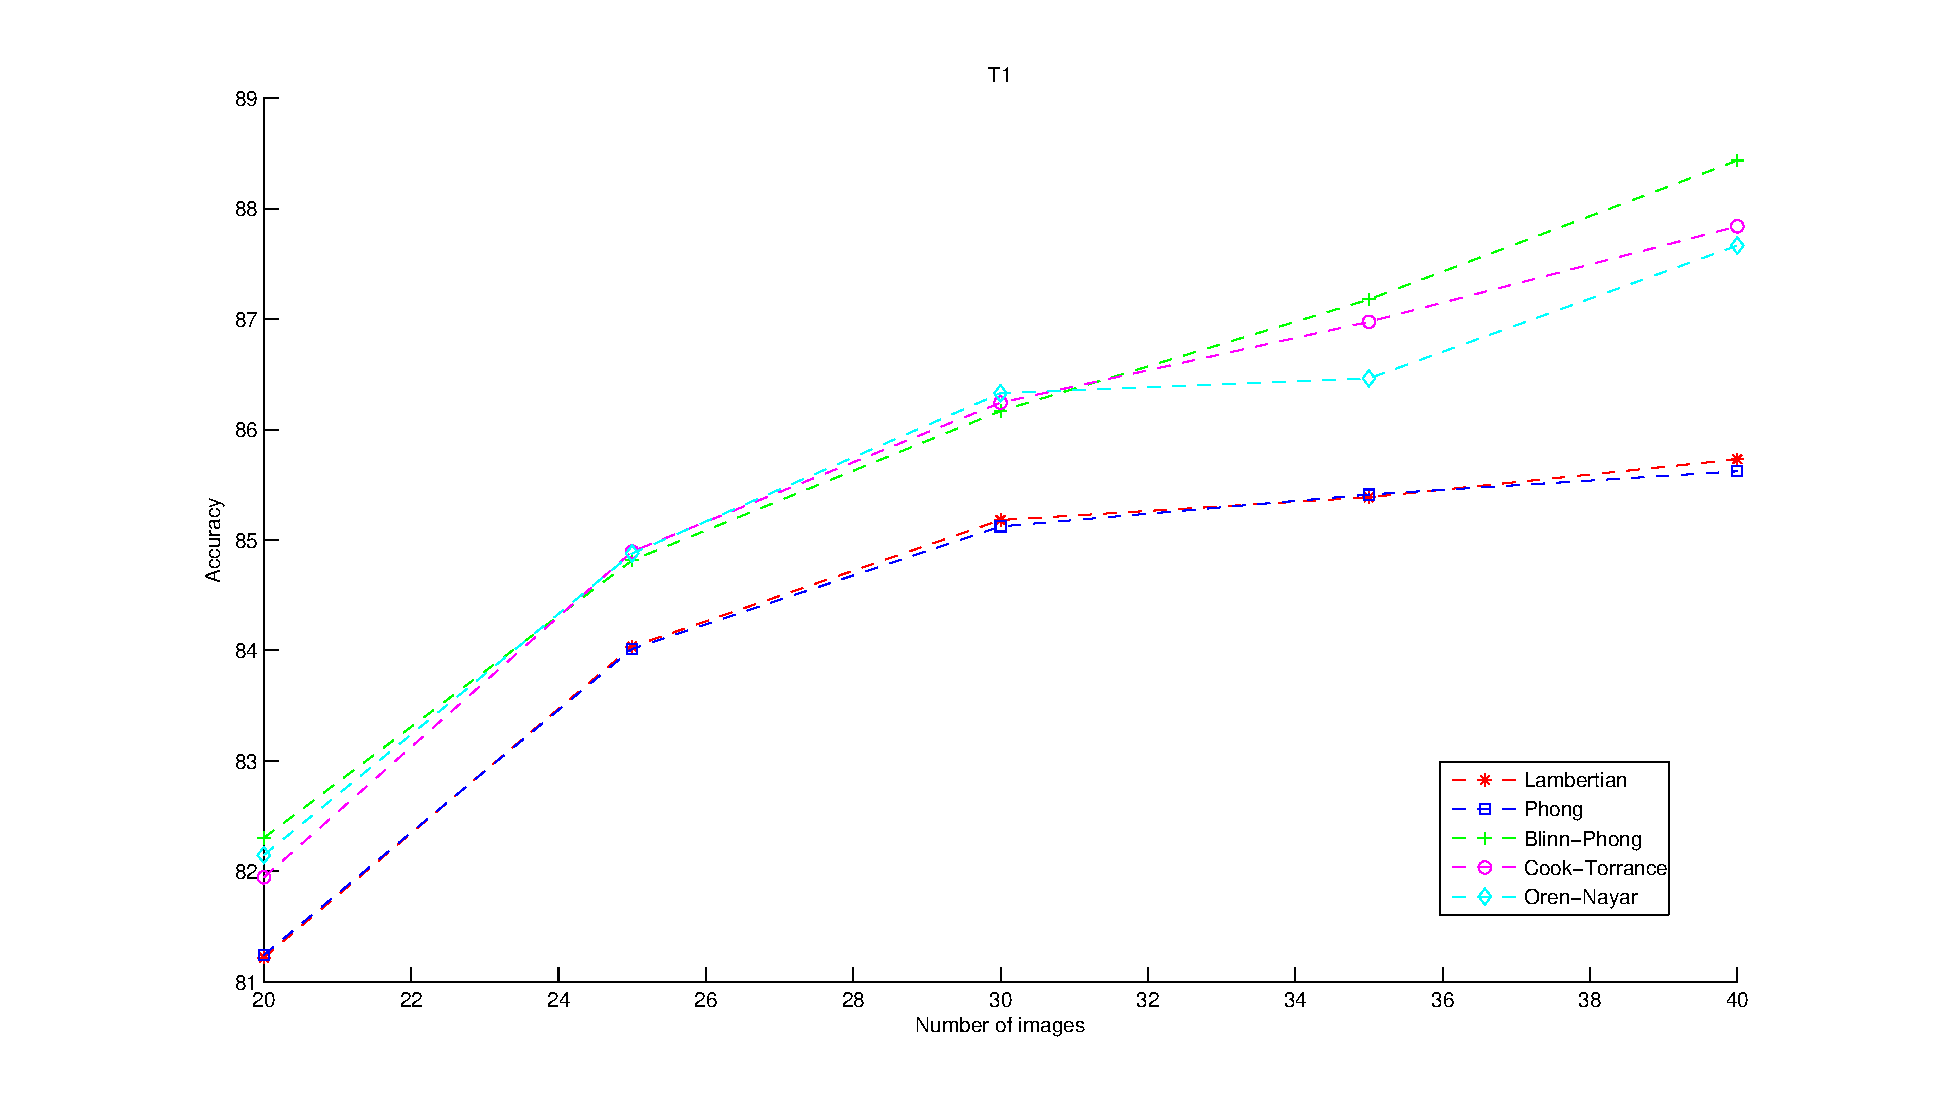
\epsfig{file=images/results/T1.eps, width=0.75\linewidth}}
		\subfigure[T3 dataset]{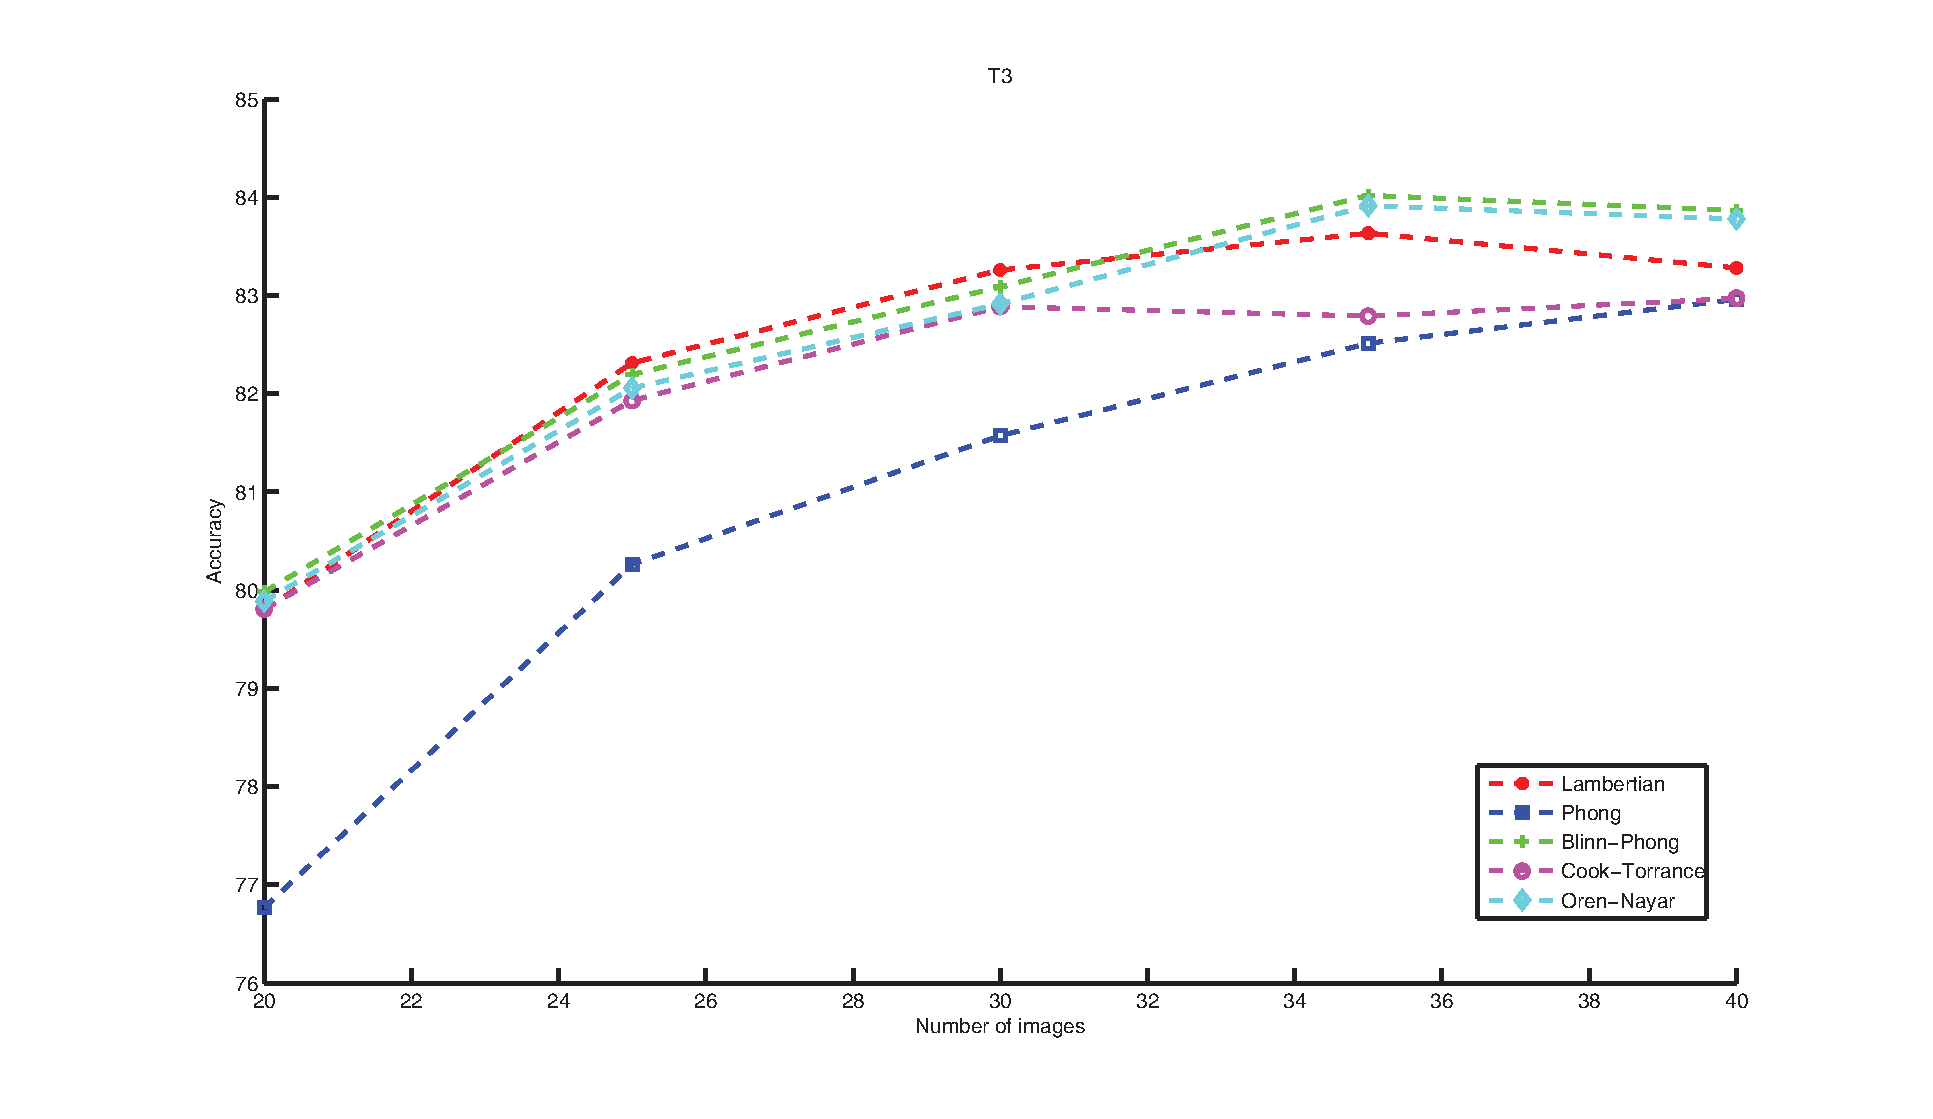
\epsfig{file=images/results/T3.eps, width=0.75\linewidth}}
		\subfigure[TT dataset]{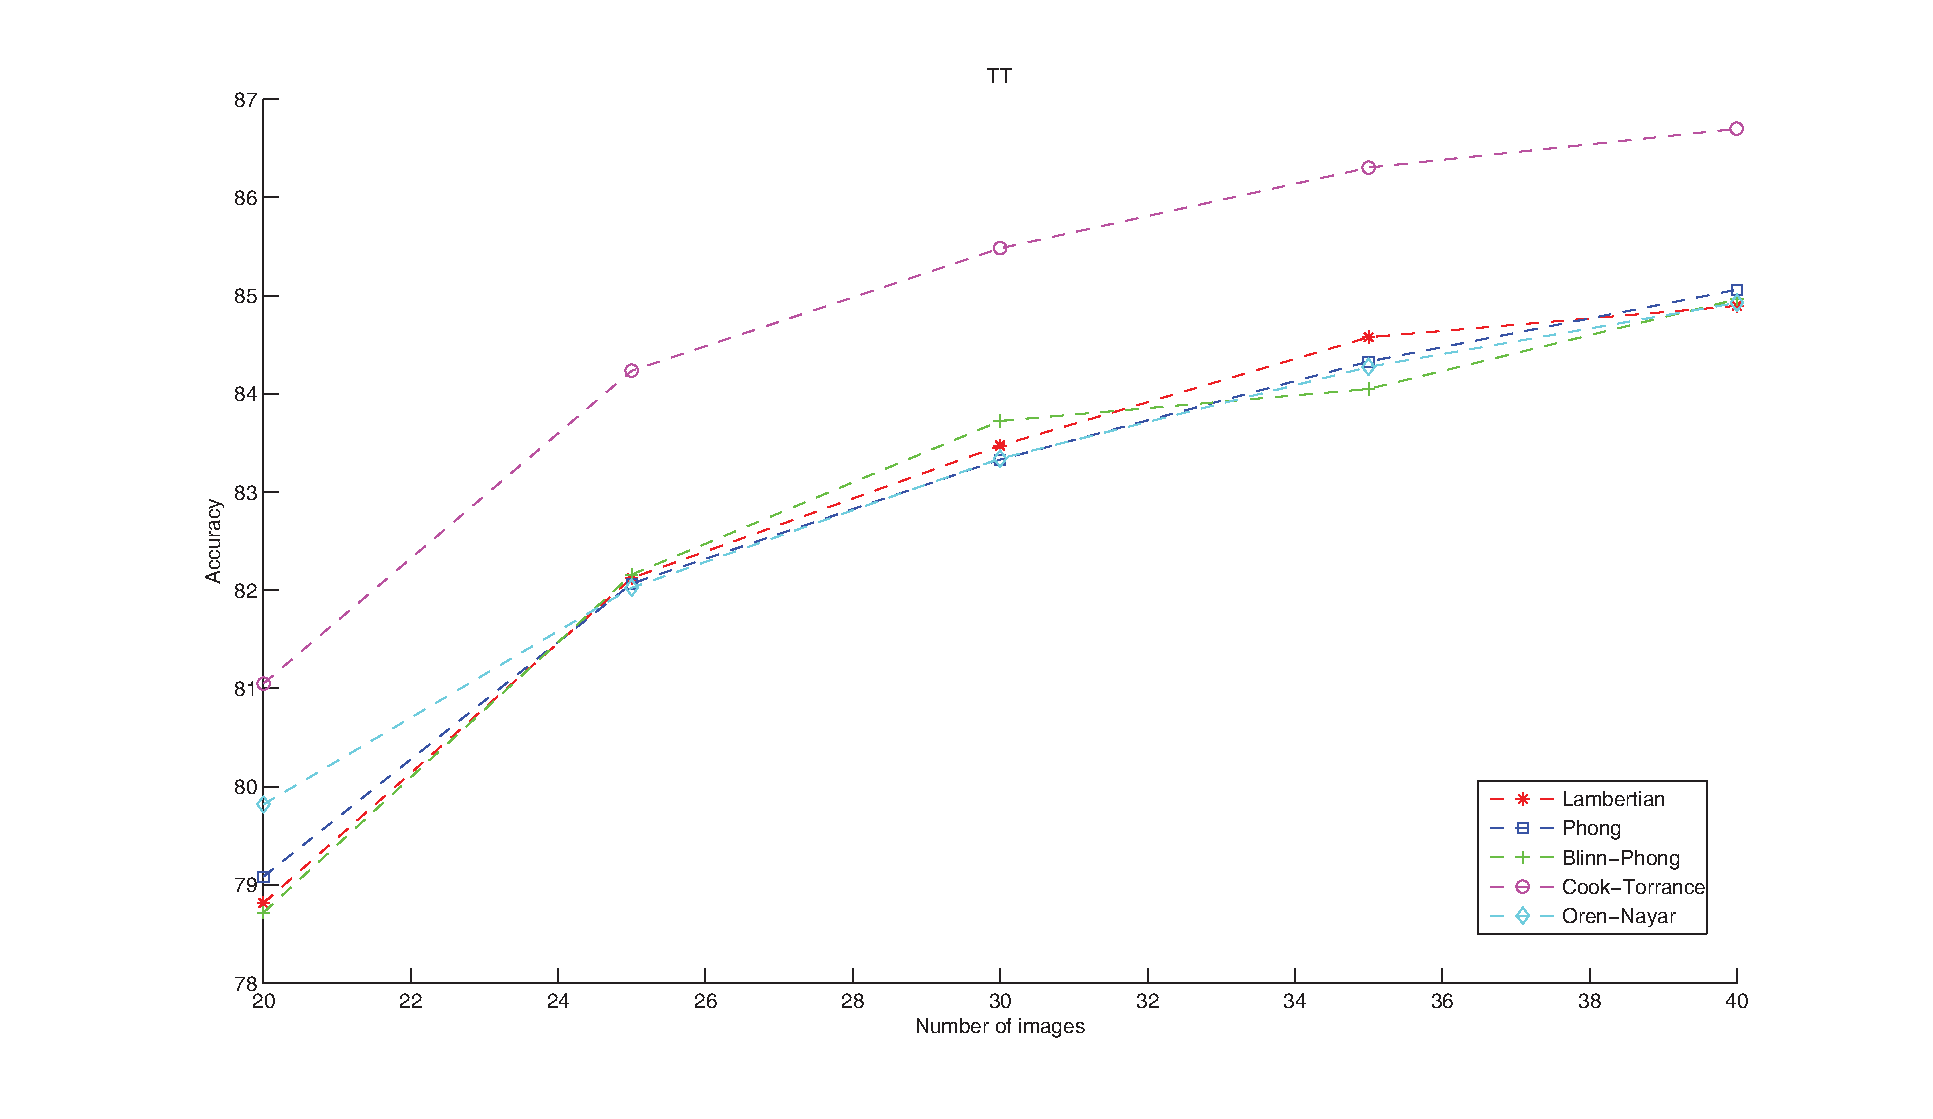
\epsfig{file=images/results/TT.eps, width=0.75\linewidth}}
	\end{center}
	\caption{{\it Results on the T1, T3 and TT dataset.}}
	\label{fig:results_A}
\end{figure}



